\section{Materiales y métodos}

\subsection{Materiales: datos generalistas}
\begin{frame}
    \frametitle{Materiales: datos generalistas (SJTU)}
    \begin{columns}
      \column{0.5\textwidth}
      \begin{enumerate}
        \item \textbf{10 nubes de puntos} de referencia.  
        \item \textbf{7} tipos de \textbf{distorsiones}: compresión, ruido al color, 
          ruido geométrico, ruido gaussiano y combinación entre ellas.
        \item \textbf{6 niveles} de intensidad.
        \item \textbf{Total de 420 nubes de puntos}.
      \end{enumerate}
      \column{0.5\textwidth}
      \begin{figure}
        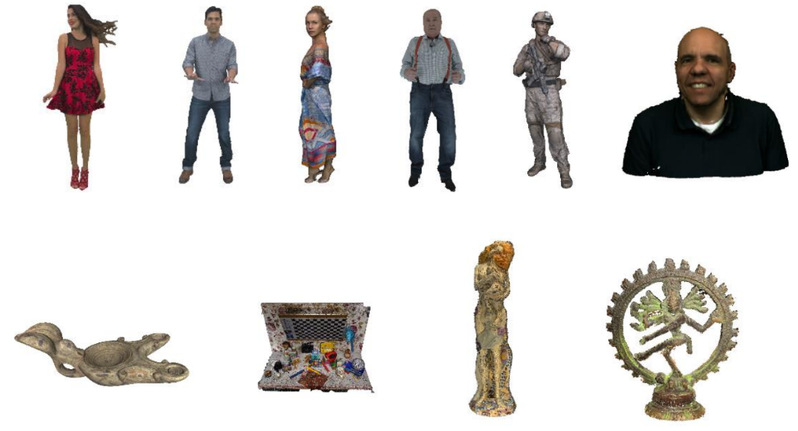
\includegraphics[width=0.95\textwidth]{imagenes/chapter3/SJTU}
        \caption{Ejemplo de conjuntos de datos SJTU\footnotemark}
        \label{fig:SJTU}
      \end{figure}
    \end{columns}
    \footcitetext{SJTU}
\end{frame}

\note{
Para el desarrollo de este proyecto, hemos hecho uso de diversos conjuntos de datos: 
El primero de ellos parte de 10 nubes de puntos 
a las cuales se aplican 7 tipos de distorsiones en 6 niveles de intensidad distintos. 
Luego, se obtiene una opinión media o MOS por sus siglas en inglés 
de 10 individuos para las 420 nubes de puntos. 
Dicho MOS sirve como medida de calidad de las mismas y para evaluar las 
predicciones del modelo. Es el procedimiento habitual.

}

\begin{frame}
    \frametitle{Materiales: datos generalistas (WPC)}
    \begin{columns}
      \column{0.5\textwidth}
      \begin{enumerate}
        \item \textbf{25 nubes de puntos} de referencia.  
        \item \textbf{5} tipos de \textbf{distorsiones}: 
          sumuestreo, ruido gaussiano, \emph{trisoup}, V-PCC y \emph{octree}.
        \item Longitud de \textbf{intensidades variantes}.
        \item \textbf{Total de 741 nubes de puntos}.
      \end{enumerate}
      \column{0.5\textwidth}
      \begin{figure}
        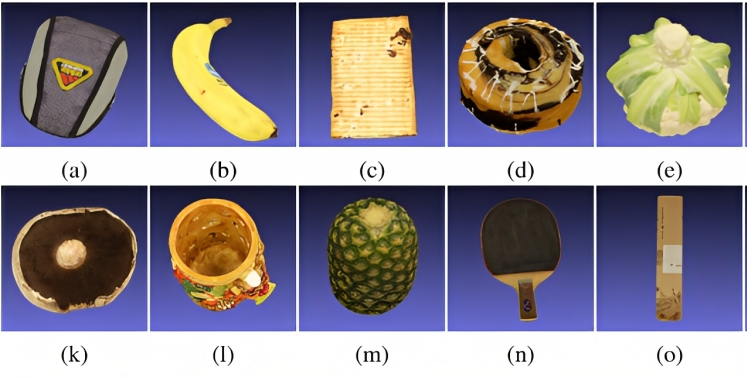
\includegraphics[width=.95\textwidth]{imagenes/chapter3/WPC}
        \caption{Ejemplo de conjuntos de datos WPC\footnotemark}
        \label{fig:WPC}
      \end{figure}
    \end{columns}
    \footcitetext{WPC1}
\end{frame}

\note{
A continuación uno similar: WPC, pero en este caso tenemos más nubes de puntos 
de partida y, mayoritariamente, distorsiones de compresión. Los niveles de 
distorsión dependen del tipo de compresión. En total tendremos 741 nubes de puntos. 
}

\begin{frame}
  \frametitle{Materiales: datos generalistas (LS-PCQA)}
  \begin{columns}
    \column{0.5\textwidth}
    \begin{enumerate}
      \item \textbf{104 nubes de puntos} de referencia.  
      \item \textbf{31} tipos de \textbf{distorsiones}.
      \item \textbf{7 niveles} de intensidad.
      \item \textbf{Total de 22000 nubes de puntos}.
    \end{enumerate}
    \column{0.5\textwidth}
    \begin{figure}
      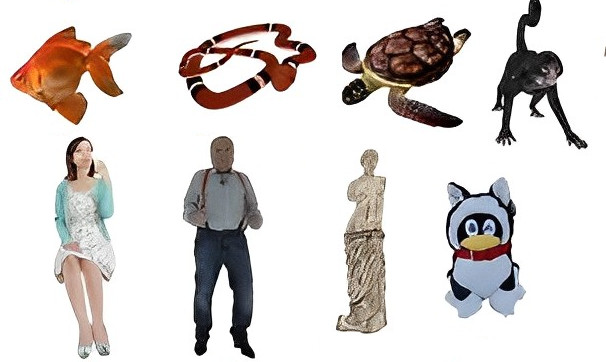
\includegraphics[width=0.8\textwidth]{imagenes/chapter3/LSPCQA}
      \caption{Ejemplo de conjuntos de datos LS-PCQA\footnotemark}
      \label{fig:LSSJTU}
    \end{figure}
  \end{columns}
  \footcitetext{ResSCNN}
\end{frame}

\note{
Luego, tenemos el reciente conjunto de datos sintético publicado en 2022.
Dicho conjunto de datos es considerado el mayor hasta la fecha, llegando a un 
total de 22000 nubes de puntos con 31 tipos de distorsiones distintas a 7 niveles 
de intensidad. 
}

\subsection{Materiales: datos sintéticos}
\begin{frame}
  \frametitle{Materiales: datos sintéticos}
  \vspace{-.8cm}
    \begin{figure}[htp]
      \subfloat[]{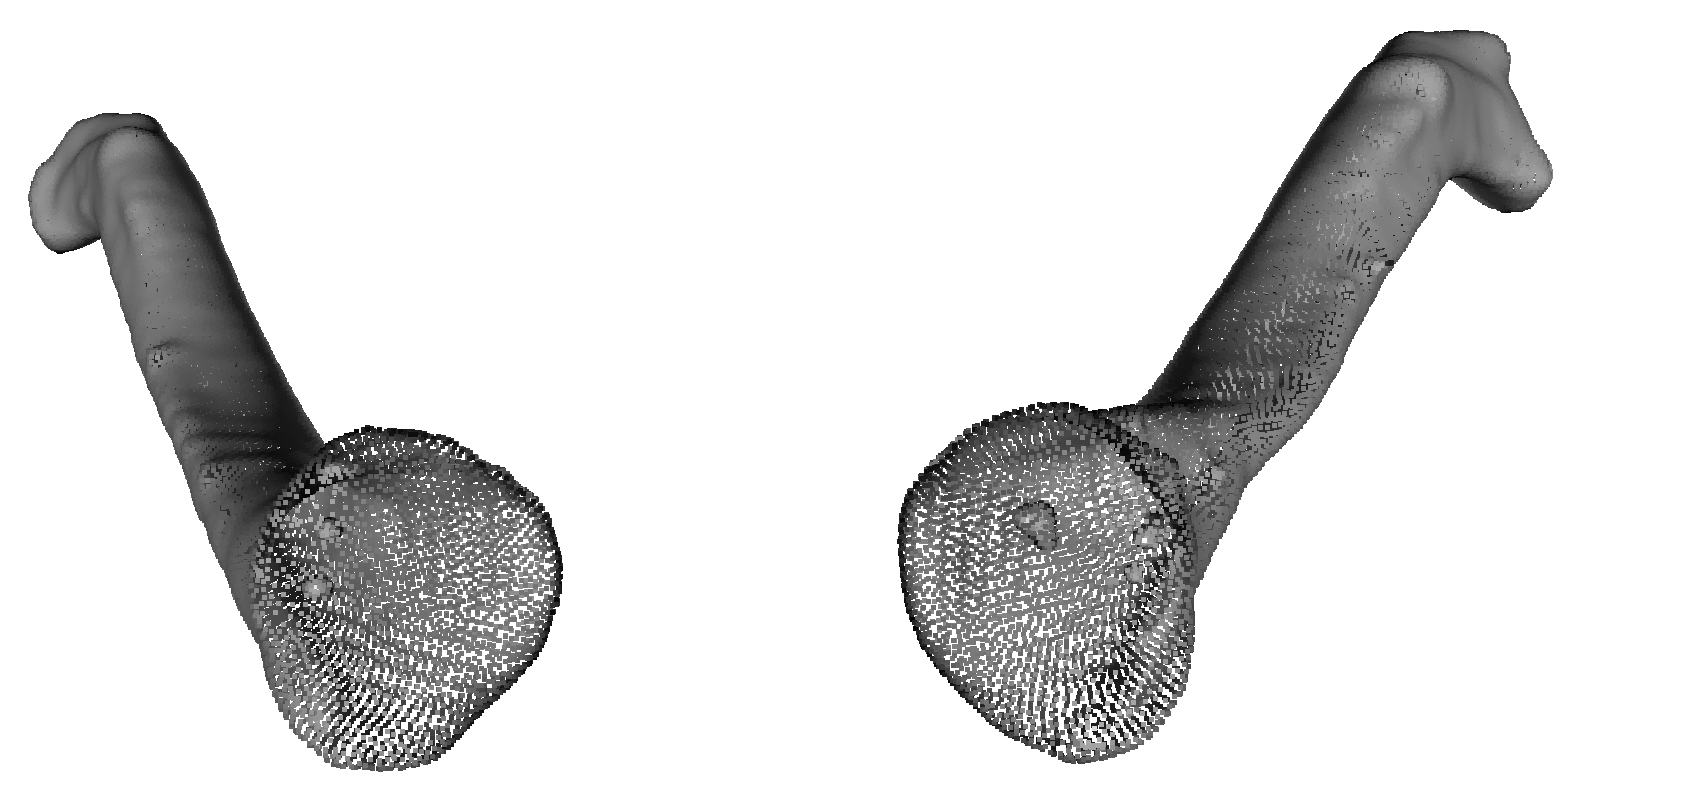
\includegraphics[width=.3\textwidth]{imagenes/chapter3/clavicula/clavicula_0.png}}
      \subfloat[]{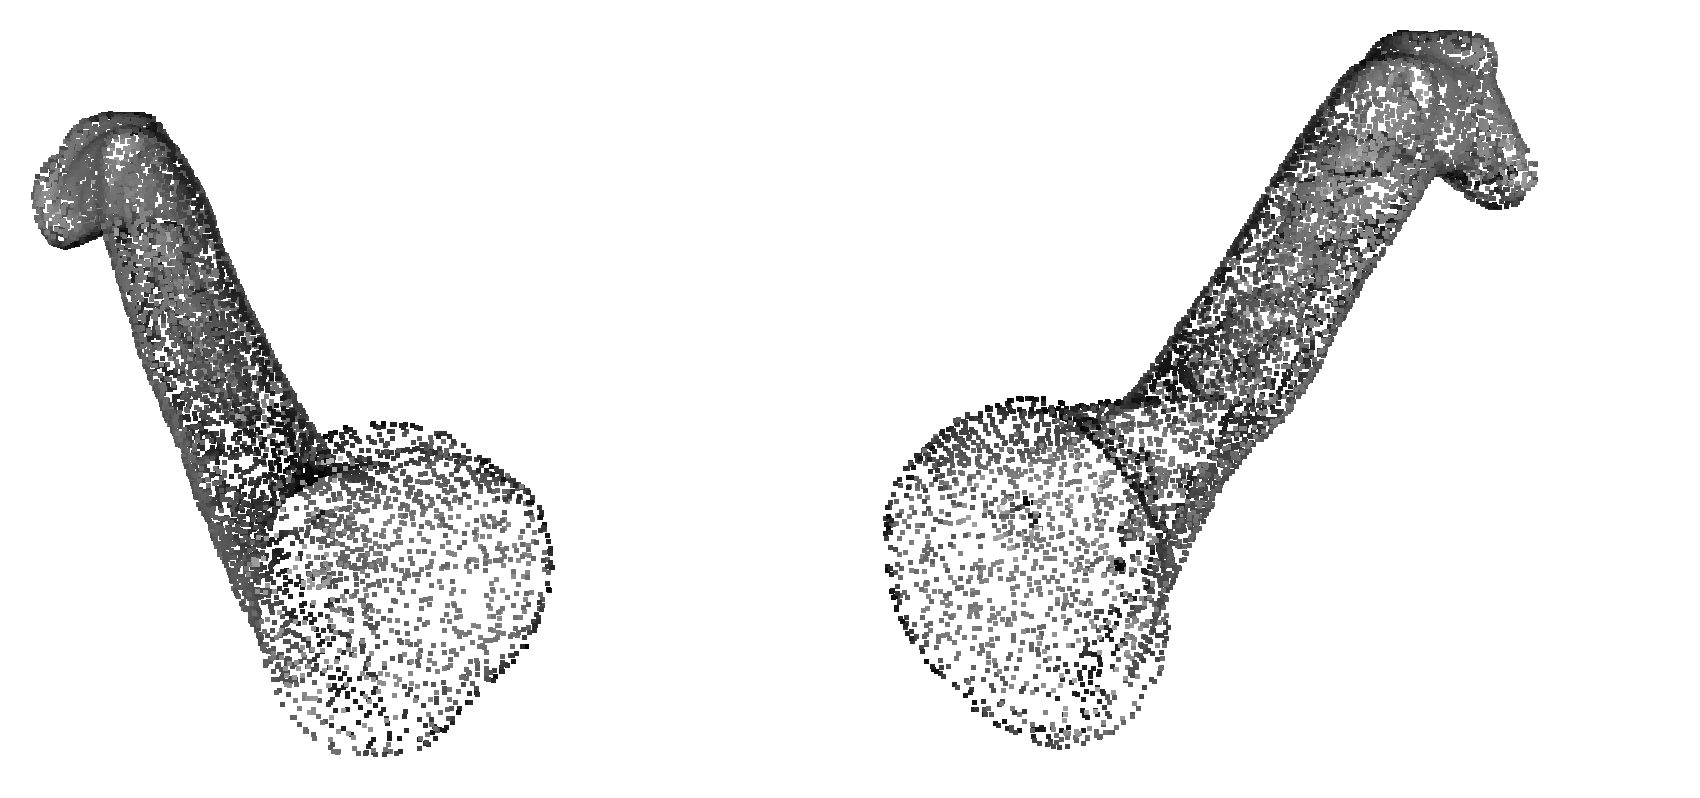
\includegraphics[width=.3\textwidth]{imagenes/chapter3/clavicula/clavicula_2.png}}
      \subfloat[]{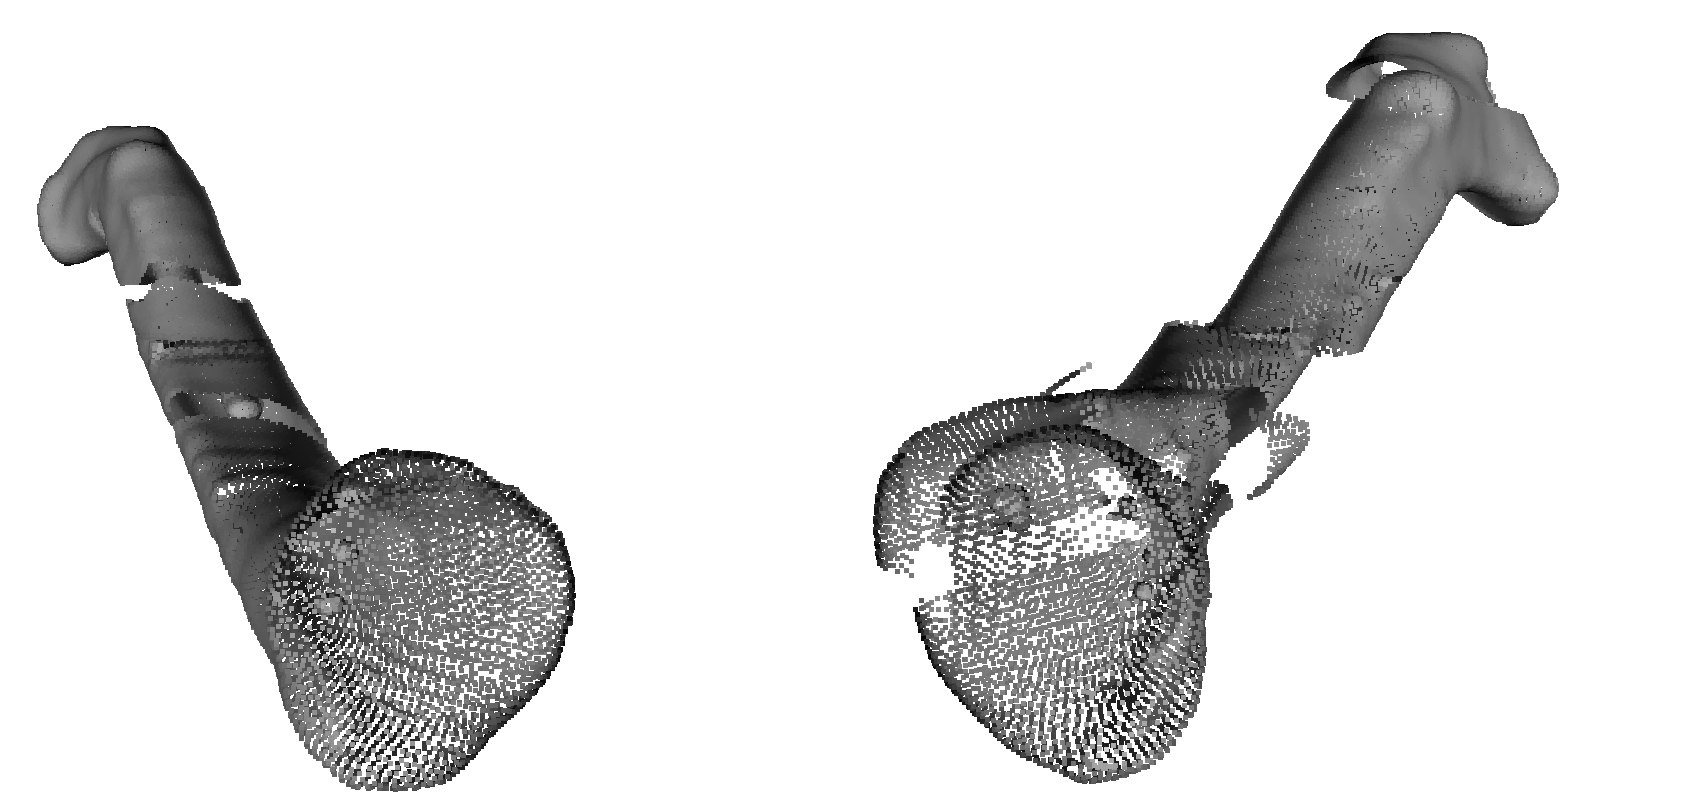
\includegraphics[width=.3\textwidth]{imagenes/chapter3/clavicula/clavicula_3.png}}
      \caption{Ejemplo de distorsiones generadas sobre clavículas, donde (a) es la imagen original, 
      (b) la distorsionada por submuestreo y (c) por movimiento local.}
      \label{fig:DistorsionesGeneradas}
    \end{figure}
  \vspace{-.3cm}
    \begin{enumerate}
      \item \textbf{11 nubes de puntos} de referencia.  
      \item \textbf{5} tipos de \textbf{distorsiones}: 
        submuestreo, compresión, ruido, rotación y movimiento local.
      \item \textbf{7 niveles} de intensidad para un \textbf{total de 385 nubes de puntos}.
    \end{enumerate}
\end{frame}

\note{
Por último, 
para la validación sobre un conjunto de datos médicos fue necesaria la creación 
de un conjunto de datos sintético. La razón es que 
no existe un conjunto de datos públicos para este análisis. 
Para ello estudiamos y fabricamos las 
distorsiones más comunes del ámbito biomédico con respecto a las reconstrucciones 3D. 
Disponemos de 11 nubes de puntos originales, 
sobre las cuáles se simulan 5 tipos de distorsiones 
a 7 niveles de intensidad cada una. Para un total de 385 representaciones.
En las distorsiones se simula tanto errores de transmisión, 
compresión, como el movimiento del paciente.
}

\begin{frame}
  \frametitle{Materiales: Generación de etiquetas}
  \begin{enumerate}
    \item Evitamos el problema logístico de obtención de la opinión media de calidad (MOS).
      \begin{itemize}
        \item Evaluación manual por grupo de personas en un entorno controlado.
      \end{itemize}
    \item Hacemos uso de las mejores métricas con referencia.
      \begin{itemize}
        \item Desglosamos el rendimiento por tipo de distorsión.
      \end{itemize}
  \end{enumerate}
\begin{table}
  \centering 
  \scriptsize
  \begin{tabular}{|c|c|c|}
    \hline
    \rowcolor[HTML]{FFC702}
     & \textbf{Parte I} & \textbf{Parte II} \\
    \hline 
    SROCC & 0.902697 & 0.878517\\
    \hline
    PLCC & 0.910713 & 0.871917\\
    \hline
  \end{tabular}
  \caption[Correlación de métricas sintéticas.]{
    Correlación de métricas sintéticas con experimento subjetivo de Liu et al\footnotemark[8].
}
  \label{tab:PseudoCorr}
\end{table}
\footnotetext[8]{\cite{ResSCNN}}
\end{frame}

\note{
Para evitar el problema logístico del etiquetado a través de la 
evaluación humana sobre el dataset sintético, 
fue necesario estudiar el problema PCQA con referencia y hacer uso de las métricas 
más empleadas. 
Dichas métricas demostraron una alta correlación con el sistema visual humano, 
justificando así su uso para generar etiquetas artificiales.
Para ello, agrupamos las mejores métricas por tipo de distorsión al igual 
que en el trabajo de Liu y sus colaboradores. Donde, en la tabla inferior, 
se puede observar la alta correlación de las etiquetas sintéticas 
en dos conjuntos de validación, ya que los valores son cercanos a 1 o 100\%. 
Parte I es el conjunto usado para elegir las métricas y Parte II un conjunto distinto.
}

\begin{frame}
  \frametitle{Métricas}
  \begin{adjustwidth}{-.5cm}{}
  \begin{table}
      \setlength{\tabcolsep}{12pt}
  \begin{tabular}[l]{cc}
        \textbf{Correlación lineal de Pearson (PLCC)} 
        &
        \textbf{Correlación de rangos de Spearman (SROCC)} 
        \\
        \parbox[c]{6cm}{ 
   \centering
          $
  PLCC(x,y) = \frac{\sum_{i=1}^m (x_i - \bar x)(y_i - \bar y)}{\sqrt{\sum_{i=1}^m (x_i - \bar x)^2}\sqrt{\sum_{i=1}^m (y_i - \bar y)^2}}
        $ 
        \vspace{.3cm}
    }
& 
\parbox[c]{6cm}{
   \centering
   \vskip5pt
  $
  SROCC(x,y) = \frac{\sum_i (x_i - \bar x)(y_i - \bar y)}{\sqrt{\sum_i (x_i - \bar x)^2}\sqrt{\sum_i (y_i - \bar y)^2}}
        \vspace{.3cm}
$
}
\\ 
\parbox[c]{5cm}{
  \centering
  \footnotesize
    Evalúa si existe una \textbf{relación lineal} entre conjuntos. 
    \vspace{.5cm}
}
&
\parbox[c]{5cm}{
  \centering
  \footnotesize
  Evalúa la relación lineal entre los \textbf{\emph{rankings}}.
  \vspace{.5cm}
}
      \end{tabular}
  \end{table}
\end{adjustwidth} 
\end{frame}

\note{
Las métricas visualizadas anteriomente son las medidas más utilizadas 
en el campo. Dichas métricas miden la relación entre conjuntos, pongamos 
x para el valor real e y para el valor predicho. 
Estas son correlación lineal de Pearson y la de rangos de Spearman.
Dichas métricas, al ser coeficientes de correlación toman valores en el intervalo [-1, 1].
Donde un valor cercano a -1 siginifica que tienen una relación inversa, 
donde una crece la otra decrece, y un valor cercano 1 indica que tienen la 
misma pendiente. 
}

\subsection{Métodos}
\begin{frame}
  \frametitle{Modelo NR3DQA\footnote[frame]{\cite{NR3DQA}}}
  \begin{columns}
    \column{0.5\textwidth}
    \begin{enumerate}
      \item \textbf{Extracción independiente} del modelo.
        \begin{itemize}
          \item Anisotropía
          \item Planaridad
          \item Esfericidad 
          \item Curvatura 
          \item Linealidad
        \end{itemize}
      \item \textbf{Descartamos} las características lumínicas.
      \item Usamos: \textbf{media, desviación y entropía}.
    \end{enumerate}
    \column{0.5\textwidth}
    \begin{figure}
      \begin{center}
        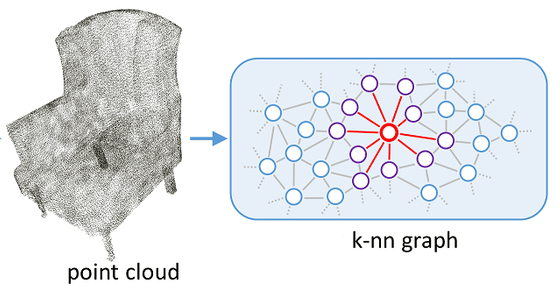
\includegraphics[width=\textwidth]{imagenes/chapter3/PatchSelection}
      \end{center}
      \caption{Extracción de características del vecindario.}
    \end{figure}
    \end{columns}
\end{frame}

\note{
Antes de probar directamente con modelos de DL, experimentamos con un método de 
ML. Dicho método está basado en la extracción de características de escena y entrenamiento de un 
modelo de vectores soporte para la regresión. 
Zhang y sus colaboradores proponen utilizar características geométricas y de 
color. Para la primera, extraen la curvatura, 
anisotropía, linealidad , 
planaridad y esfericidad de los puntos. 
Estas características se pueden extraer del vecindario 
de un punto por medio de la matriz de covarianza y los valores singulares 
de los K-vecinos más cercanos. Se calcularan para todos los puntos. 
Utilizaremos los valores medios, desviación y la entropía de estas características.
Además, calcularemos sus distancias a las distribuciones gaussiana y gamma, 
dado que se observó que la distribución de estas se veía afectada por la intensidad 
de las distorsiones. 
Las características lumínicas la descartamos, 
ya que información de textura o color no existe en los volúmenes
médicos habituales. 

}

\begin{frame}
  \frametitle{Modelo VQA-PC\footnote[frame]{\cite{VQA-PC}}}
  \begin{columns}
    \column{0.5\textwidth}
    \begin{enumerate}
      \item \textbf{Extracción automática} de características.
      \item Extracción \textbf{espacial y temporal} de las reconstrucciones.
        \begin{itemize}
          \item Espacial por fotogramas estáticos de \textbf{distintas perspectivas}.
          \item Temporal por tratar la \textbf{nube como video}.
        \end{itemize}
      \item Es como un \textbf{meta-modelo} de aprendizaje profundo. 
    \end{enumerate}
    \column{0.5\textwidth}
    \begin{figure}
      \begin{center}
        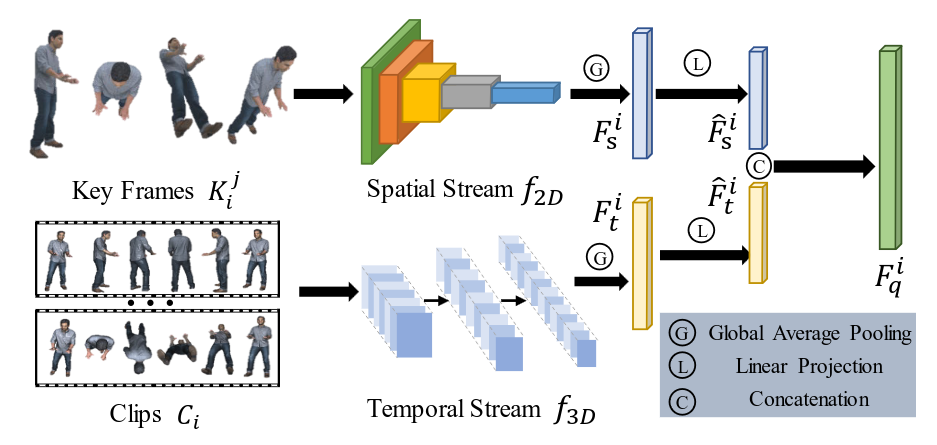
\includegraphics[width=\textwidth]{imagenes/chapter3/PipelineCompleto}
      \end{center}
      \caption{Estructura del modelo VQA-PC\footnotemark[10]}
    \end{figure}
  \end{columns}
\end{frame}

\note{
Por otro lado, en DL se propone un modelo de estimación de calidad de nubes 
de puntos utilizando proyecciones 2D, pero desde múltiples perspectivas. 
Zhang y sus colaboradores argumentan que los métodos anteriores de proyección 
se basan en la hipótesis de que los humanos percibimos la calidad de modelos 
3D desde una perspectiva estática, cosa que no 
es cierta en la práctica dado que los objetos 3D permiten operaciones geométricas 
de rotación y escalado.
Y por ello, siguiendo la motivación de que las deformaciones geométricas 
no deseados se presentan de forma abrupta según la perspectiva, proponen 
unificar la percepción estática con la dinámica tratando 
a las nubes de puntos como vídeos del objeto 3D rotando.
}

\subsection{Entorno}
\begin{frame}
  \frametitle{Tecnologías utilizadas}
  \begin{table}[htp]
    \vspace{-.5cm}
      \begin{tabular}{cccc}
        \begin{minipage}{.2\textwidth}
          
\includegraphics[width=\textwidth]{imagenes/chapter3/Python}
        \end{minipage} 
                                  & 
        \begin{minipage}{.2\textwidth}
          
\includegraphics[width=.9\textwidth]{imagenes/chapter3/FastAI}
        \end{minipage} 
                                  & 
        \begin{minipage}{.2\textwidth}
          
\includegraphics[width=\textwidth]{imagenes/chapter3/Pytorch}
        \end{minipage} 
                                  &
        \begin{minipage}{.2\textwidth}
          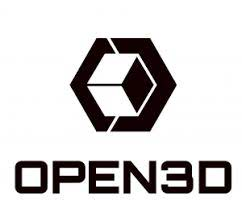
\includegraphics[width=.9\textwidth]{imagenes/chapter3/Open3D}
        \end{minipage} 
                                  \\
        \begin{minipage}{.2\textwidth}
          
\includegraphics[width=\textwidth]{imagenes/chapter3/Numpy}
        \end{minipage} 
                                                        & 
        \begin{minipage}{.2\textwidth}
          
\includegraphics[width=.9\textwidth]{imagenes/chapter3/Scikit}
        \end{minipage} 
                                                        & 
        \begin{minipage}{.2\textwidth}
          
\includegraphics[width=.9\textwidth]{imagenes/chapter3/Polars}
        \end{minipage} 
        &
                                                        \\
                                                        & 
        \begin{minipage}{.2\textwidth}
          
\includegraphics[width=.9\textwidth]{imagenes/chapter3/Nvidia}
        \end{minipage} 
                                                        & 
        \begin{minipage}{.2\textwidth}
          
\includegraphics[width=.9\textwidth]{imagenes/chapter3/Colab}
        \end{minipage} 
                                                        &
                                                        \\
      \end{tabular}
  \end{table}
\end{frame}

\note{
Para el desarrollo y ejecución de los modelos fue necesario el uso de
la librería de DL Pytorch junto con las librerías CUDA para poder ejecutar 
los modelos en las tarjetas gráficas de NVIDIA. Para los cálculos numéricos y 
el manejo de datos se utilizaron Numpy y Polars. Teniendo en cuenta que para el
cálculo de las métricas hemos utilizado la librería de scikit-learn.
Para la visualización y fácil manipulación de las nubes de puntos se hizo uso 
de la librería de Open3D y Pyntcloud.
}
